%!TEX root =  main.tex
%!TEX encoding = UTF-8 Unicode
\chapter{データの入力}
\label{sec:getpref}

ここでは,推薦システムの実行過程の最初の段階である「データの入力」について述べる.
この段階では,活動利用者に自身の嗜好データを,推薦システムへ入力させる.
嗜好データとは,利用者の各アイテムへの関心や好みの度合いをを数量化したものである.
システムによっては,この嗜好データの代わりに,活動利用者に検索質問や批評を入力させるものもある.
この検索質問は,アイテムの特徴についての制約条件を具体的に記述したものである.
例えば,レストランの推薦システムで,価格帯や,和洋中の別などを具体的に指示するために「価格は6000円以下で,和食の店」といった形式の検索質問を入力する.
こうした検索質問は,情報検索やデータベースのクエリ検索の技術がほぼ転用できるので,ここでは,嗜好データについて述べる.
さらに,これら嗜好データや検索質問で表された,活動利用者の嗜好パターンの以外のデータも推薦システムは利用する.
このようなデータとして,活動利用者以外の利用者の嗜好データ,アイテムの特徴,利用者の年齢や性別などの情報,現在位置などの利用状況を示す情報などがあり,これらにつても述べる.
なお,嗜好データの収集全般については,文献\cite{jjsai:04:05}にまとめられている.
また,文献\cite{sigir:01:01}は,推薦システムの利用者へのアンケート調査結果に基づいて,入力インタフェースについての設計指針を示している.
アイテムについての情報は,利用者が評価するときに見えるようにしておくと,システムへの満足が高まると報告している.

\section{暗黙的と明示的な嗜好データの獲得}
\label{sec:getprefimpexp}
\index{嗜好データ}\index{preference data}

\begin{table}
\centering
\caption{嗜好データ獲得法の長所と短所}
\label{tab:getprefcomp}
\begin{tabular}{l@{\qquad}c@{\,:\,}lc@{\,:\,}l}\toprule
 & \multicolumn{2}{c}{明示的} & \multicolumn{2}{c}{暗黙的} \\\midrule
データ量       & × & 少ない & ○ & 多い \\
データの正確さ & ○ & 正確 & × & 不正確 \\
未評価と不支持の区別 & ○ & 明確 & × & 不明確 \\
利用者の認知   & ○& 認知 & ×& 不認知\\
\bottomrule
\end{tabular}
\end{table}

まず,嗜好データを獲得するアプローチは,おおきく暗黙的と明示的の二種類に分けられる.
明示的な獲得とは,利用者に好き嫌いや,関心のあるなしを質問し,利用者に回答してもらう方法である.
もう一方の暗黙的な獲得とは,利用者の行動をから,利用者の嗜好や関心を推察することで嗜好データを得る方法である.
例えば,購入したり,閲覧したりしたアイテムには,利用者は関心があるとみなしたりする.

まず,二つの嗜好データの獲得法を比較する.
これらの獲得法の長所と短所を\ref{tab:getprefcomp}にまとめた.
データ量については,利用者の嗜好の予測には統計的な方法が用いられるので,予測を正確にするにはより多くのデータを収集できた方が有利となる.
しかし,質問に答えるといった手間を利用者は嫌うことが多いため,明示的な獲得では多数のデータの収集は難しい.
よって,これらの点では暗黙的な手法が有利である.

データの正確さについては,暗黙的な獲得では,誤ってクリックしてしまったとか,人に頼まれて購入したなどの理由で,本当は関心がないものも,関心があるとみなされてしまう場合がある.このため,収集されたデータの正確さにおいては明示的な獲得が優れている.

利用者に明示的に評価してもらう場合では,アイテムを利用者が評価したかどうかはもちろん明確である.
しかし,暗黙的な評価では,利用者がそのアイテムに対して積極的な行動をしなかったことをもって,そのアイテムへの不支持とみなす場合がある.
例えば,閲覧しなかったアイテムは好きではないとみなしたとする.
このとき,アイテムについて未評価であることと不支持であることの区別ができない.
場合によっては,閲覧していないために,利用者が好むアイテムを嫌いだとシステムがみなすこともある.

最後の利用者の認知とは,利用者が自分の嗜好データをいつ,どのように取得されたかを知っているかどうかということである.
システムが提示した推薦は,利用者がその根拠を把握していた方が受け入れられやすい.
暗黙的な獲得では,嗜好データを意識的に入力していないので,推薦が根拠なくなされたもののように感じられやすく不利である.

\section{明示的な獲得}
\label{sec:explicitrating}
\index{明示的評価}\index{explicit rating}

アイテムを利用者に提示し,利用者にそのアイテムに対する好みの度合いを答えてもらう明示的な嗜好データの獲得について詳細を述べる.

\subsubsection{評価の動機付け}

明示的な獲得法では,利用者はアイテムを評価することを面倒だと思うので,暗黙的な方法に比べて多数の嗜好データを集めにくいと述べた.
\cite{sigir:01:01}では,利用者は推薦の精度が向上するなど,評価付けによるメリットが明確であれば,ある程度の手間をかけて評価付けをするとの調査結果を報告している.
よって,利用者に評価をさせるような動機付けは重要である.

自身への推薦の精度を向上させるということは,利用者にとって主な動機付けとなる.
だが,管理者が想定するようなこの動機以外にも,自分の意見の表明をするためや,他の利用者の手助けになるということを動機とする場合もある\cite{jacm:04:01}.
これらの動機は,利用者の評価数の順位の公開などによって喚起することができる.
さらに,明示的にインセンティブを与えることも考えられる.
文献\cite{ieeem:07:05}は,情報検索の結果の順位付けに,他の利用者の評価を利用する,一時的個人化の推薦システムを提案している.
このシステムでは,市場の考えが導入され,検索結果を閲覧するには,ポイントの支払いが必要である.
閲覧する文書の,被評価数が多く,評価が高いほど多くのポイントを支払う必要がある.
一方,ポイントは,検索した結果を評価することで獲得でき,被評価数が少なく,高い評価をすると獲得ポイント数は増える.
すると,検索をするために,検索結果の評価をする必要が生じるため,積極的な評価付けが期待できる.

\subsection{採点法と格付け法}

利用者が好みの度合いを答えるには,それを測る尺度が必要になる.
好みの度合いを表す尺度として,$0\sim5$ や$-3\sim+3$ のような数値尺度を使う\term{採点法}{scoring method} や,上・中・下 や 適合・不適合 などの順序付カテゴリ尺度を使う\term{格付け法}{rating method}\cite{jb:015:00}が良く利用されている.
こうした方法は人間の聴覚や味覚などを定量的に計測する官能検査(sensory test)の分野で研究されてきた\cite{jb:016:00}.
採点法や格付け法は,単純な入力フォームを用いて,比較的多数のアイテムに対する嗜好データを得られることが利点である.

これらの方法を使ううえでの注意点を幾つか述べておく.
%まず,尺度の段階の数は,利用者が真に要求している嗜好の段階数と等し
%いことが望ましい.
文献\cite{sigchi:03:02}では,利用者は評価尺度の目盛りが細かい方を好む傾向があること,さらに,細かい評価で予測精度が向上することはないが悪くもならないことを報告している.
よって,目盛りは細かめに設定することを推奨している.
さらに,${-}3$〜${+}3$の尺度で,中立の$0$を抜いた尺度を使うと,中立の評価の多くは弱い肯定的な評価$+1$に移されること,予測評価値を見せながら評価させると,利用者はそれに「引きずられた」評価をすることも報告している.
\ref{sec:recomtask}で述べた適合アイテム発見を目的とする場合,目的に適合/不適合の2段階でも十分な場合が多いが,評価閲覧タスクでは,どれくらい不要なアイテムを除外したいかは利用者次第なので,より詳細な多段階の尺度を用いる方が良いだろう.
次に,質問の仕方にもいろいろな配慮をすべきである.
例えば,採点法では等間隔の尺度を連想させるように,等間隔の目盛りを見せるなどの工夫がある.これらの配慮については中森の\cite{jb:022:00}を参考にされたい.
%@@@ recsys:11:11:01

\subsection{評価値の揺らぎや偏り}

採点法や格付け法は大量の嗜好データを比較的に容易に得られるので多用されてきたが,当然ながら欠点もある.
先に,明示的な獲得は暗黙的な獲得と比べてより正確に利用者の嗜好を評価できると述べた.
だが,絶対的には不正確さや揺らぎがある.
真の嗜好の度合いは,脳の活動を直接観測するなどすれば将来的には計測できるであろうが,現在のところは厳密には計測できない.
そのため,揺らぎがあるかどうかの直接的な証明はできない.
よってここでは,採点法や格付け法によって計測した評価値が,真の評価値と乖離している間接的な証拠と,その乖離の原因を示す.

まず,評価値の揺らぎの証拠を示す.
官能検査の研究では,たとえ被験者が同じ評価値を与えていても,人によって嗜好の強さが違っていたりとか,時間がたつと一貫性が保たれなくなる問題があることが経験的に知られていた\cite{lncs:04:01}.
ソムリエなど訓練された被験者が,同一セッション内,すなわち,時間をあけずに連続して評価した場合でなければ,尺度を一定に保つことは難しいとされている.
嗜好データについても,一度映画を評価付けしたあと,6週間後にもう一度同じ被験者に同じ評価付けさせると,二つの評価値の間の相関は
0.83であったとの報告がある\cite{sigchi:95:01}.
文献\cite{sigchi:03:02}でも同様の報告がされている.
同一セッション内でも,寿司の嗜好について採点法で尋ねたのち,無関係な質問を幾つかしてから,下記の順位法で再び同じアイテムについて嗜好を質問すると,68.3\%の被験者の回答に不一致が観測された\cite{jpublist:043}.
これらの実験結果は,嗜好データには揺らぎがあることを示している.
他に,代表的な映画評価データにおいて,いろいろな工夫をしても,平均絶対誤差(MAE)を5段階尺度で0.73の「魔法の壁 (magic barrier)」より小さくできないことから,評価値そのものに揺らぎがあることが示唆されている\cite{jacm:04:01}.
以上のように,絶対的な評価値を使う採点法や格付け法では,被験者は,質問時期の違いなどにより揺らぎが生じるといえるだろう.

\begin{figure}
%(a) GroupLens   5.6  10.8  26.1  34.9  22.6
%(b) Amazon.com  7     5     8    20    60
%(c) 寿司        7.9   9.1  22.6  22.7  37.5
\centering
\begin{minipage}{0.6\fullwidth}
\centering
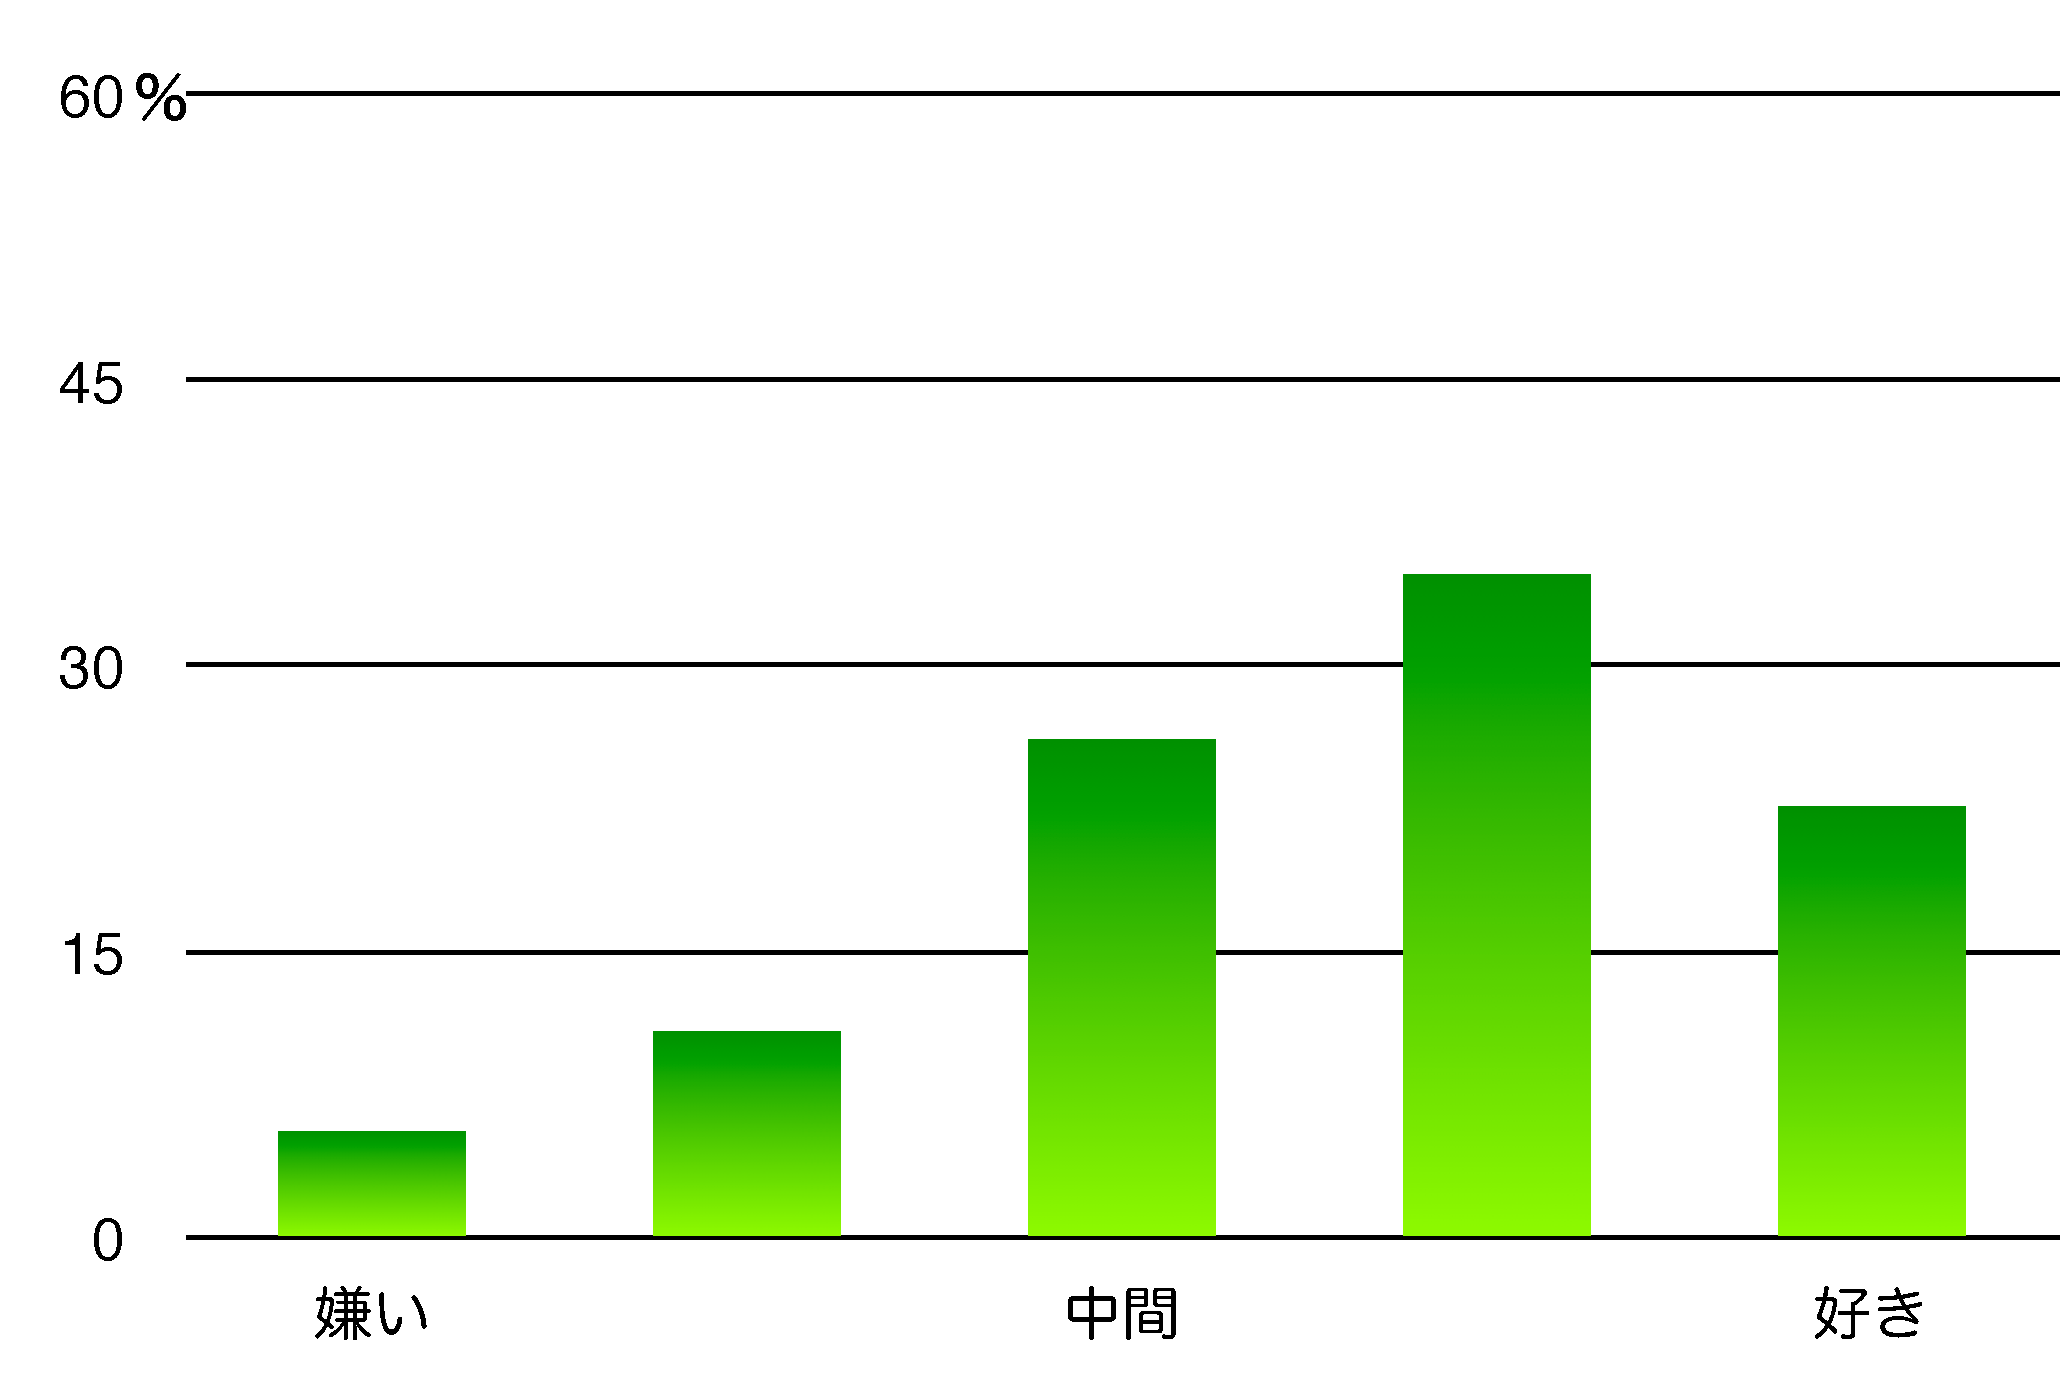
\includegraphics[width=\textwidth]{rating-score1.pdf}\\
(a)~MovieLens \cite{url:008}
\end{minipage}\\\medskip
\begin{minipage}{0.6\fullwidth}
\centering
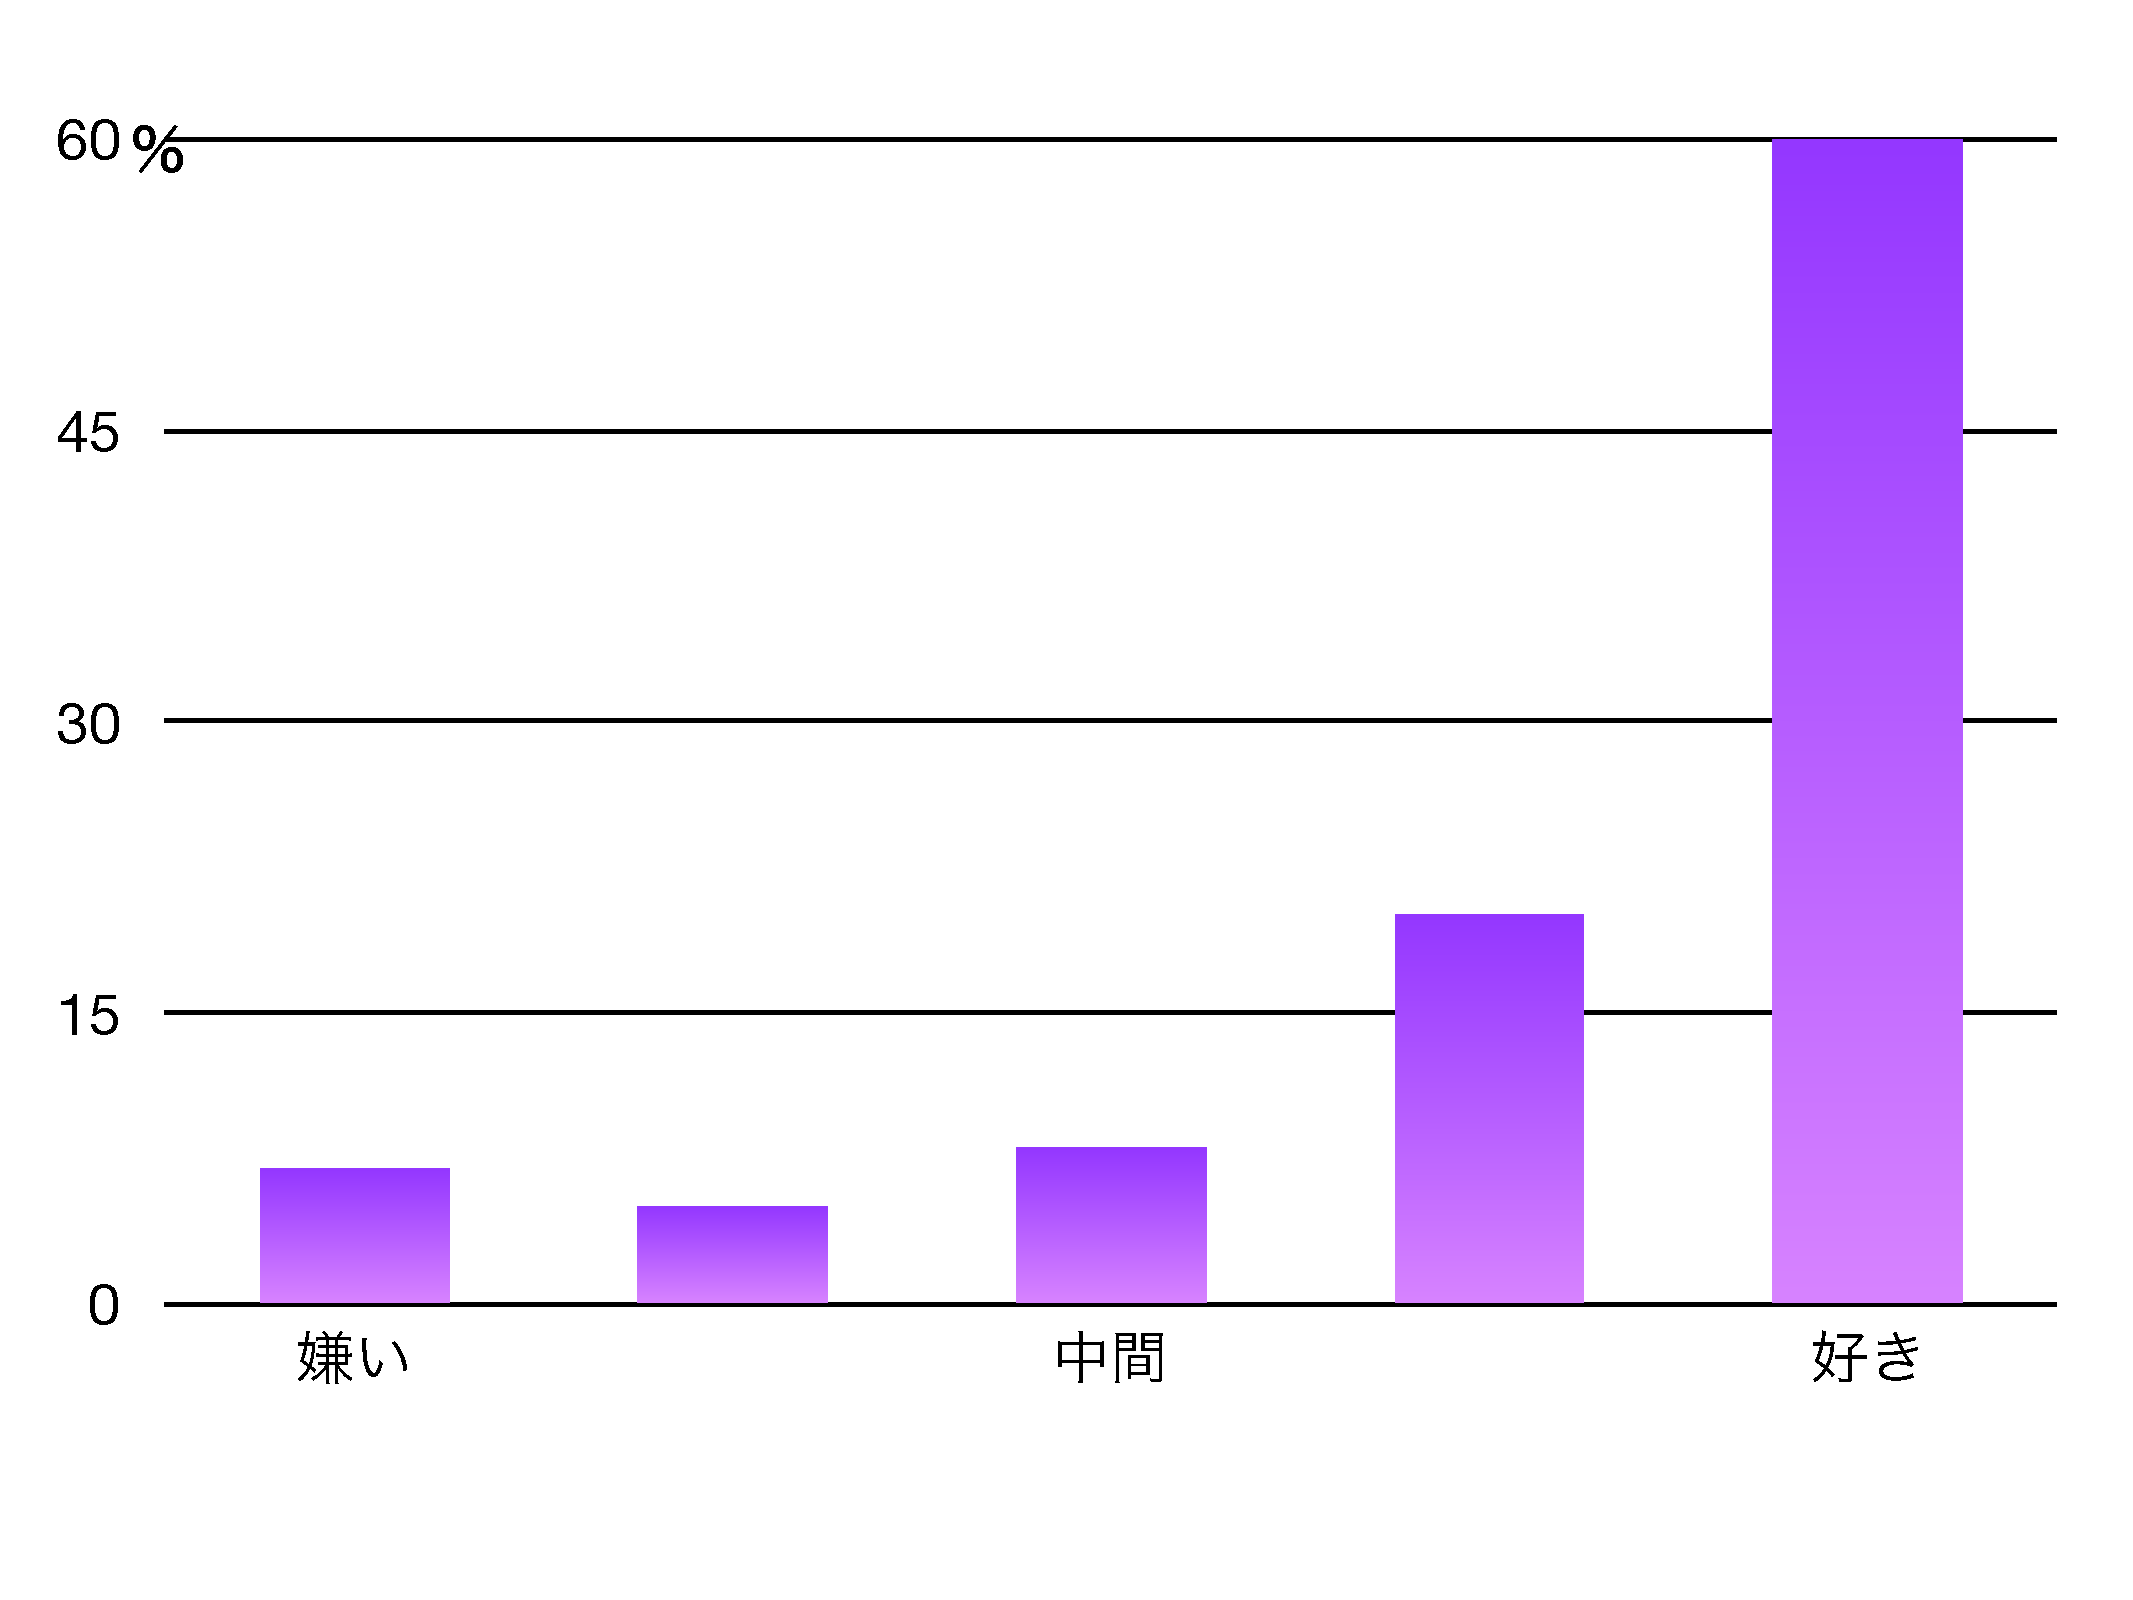
\includegraphics[width=\textwidth]{rating-score2.pdf}\\
(b)~Amazon.com \cite{misc:007}
\end{minipage}\\\medskip
\begin{minipage}{0.6\fullwidth}
\centering
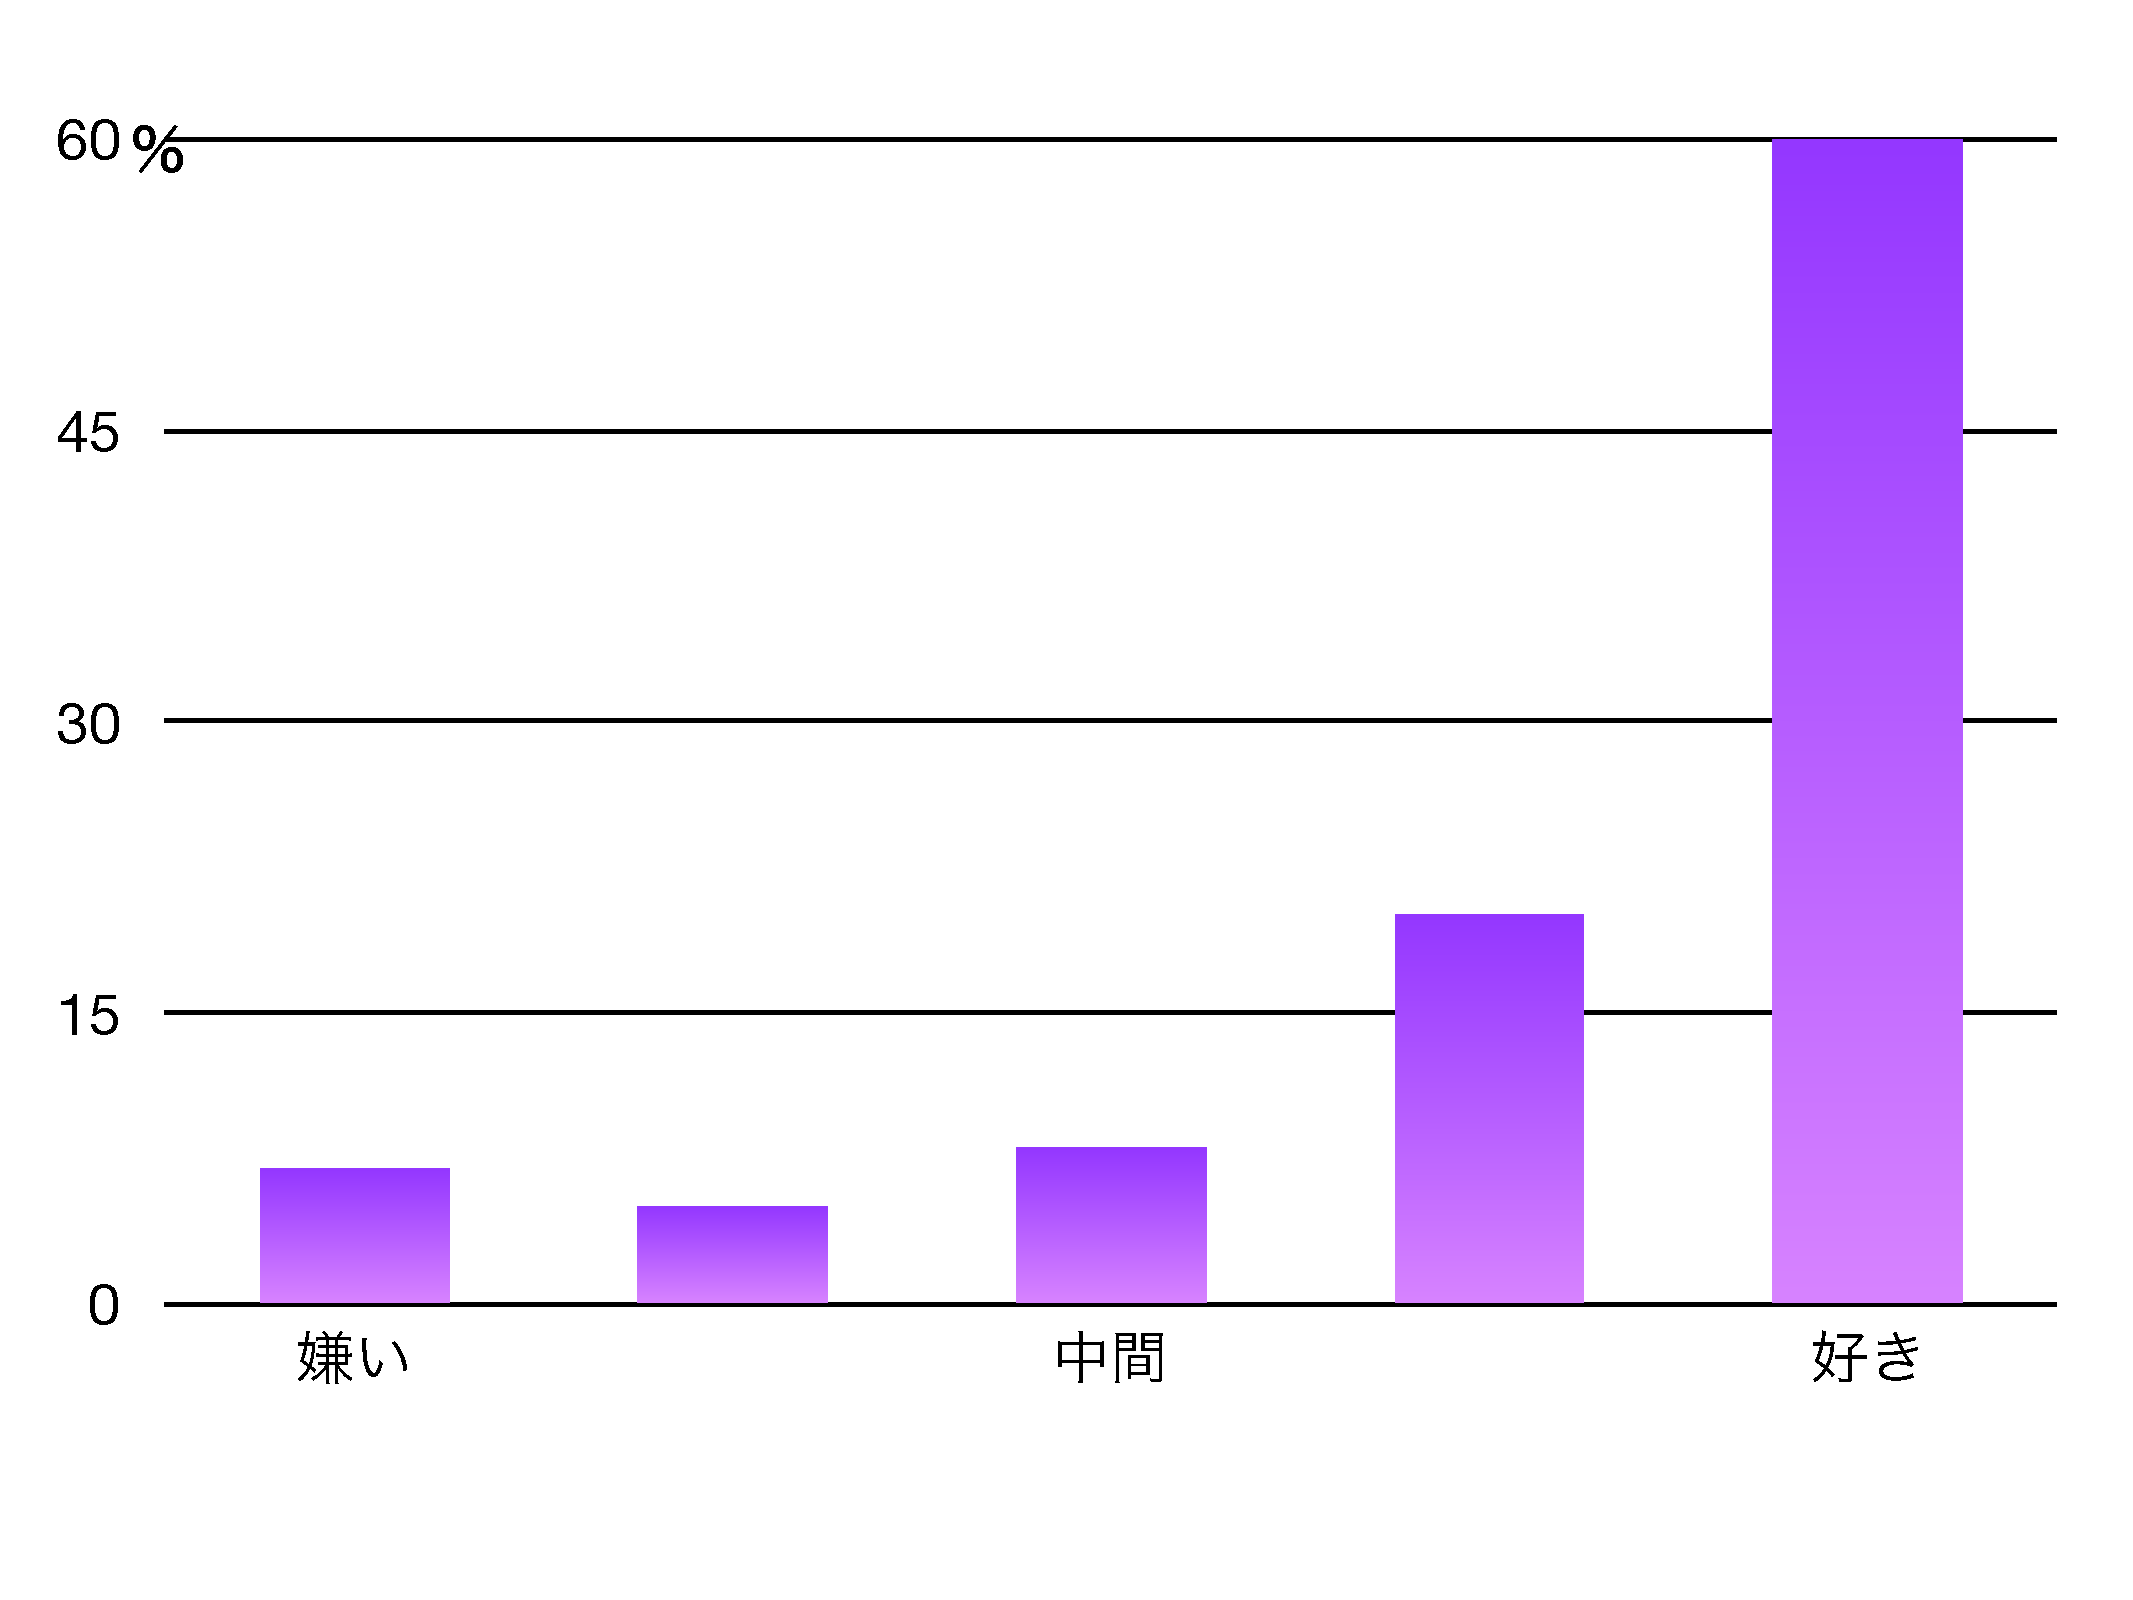
\includegraphics[width=\textwidth]{rating-score2.pdf}\\
(c)~寿司 \cite{url:020,epublist:064}
\end{minipage}
\caption{アイテムへの評価値の分布}
\label{fig:prefdist}
\end{figure}

次に,評価値の偏りについて述べる.
\ref{fig:prefdist}に,5段階の採点法を用いた3種類の嗜好データの,評価値の分布を示す.
それぞれ,(a)~MovieLensの100万要素のデータ集合\cite{url:008},
(b)~電子商取引サイトAmazon.com\cite{misc:007},(c)~寿司の嗜好調査\cite{url:020,epublist:064}での分布である.
どのデータでも,好きな方へ明らかに偏っている.
この偏りの原因には,サンプリングと真の嗜好からの乖離の二つが考えられる.
サンプリングの偏りの原因として,\ref{fig:prefdist}の(a)や(b)では,利用者が,関心がある選択的にアイテムを評価していることや,(b)や(c)では,市場の淘汰を受けて人気のあるアイテムのみが評価候補となっていることが挙げられる.
このようなサンプリングの偏りは,\ref{sec:prederr}で指摘したように,予測誤差の正確な評価を妨げる.
真の嗜好から乖離する理由としては,利用者個人がもつ心理効果の影響が考えられる.
例えば,過剰な酷評は社会的通念的に良くないとの考えをもつ人には,全体的に評価が高くする寛大効果 (leniency effect)が見られ,あいまいな判断や質問では中心のスコアを選びやすい中心化傾向 (central tendency)などが生じる\cite{jb:026:00}.
さらに,質問の仕方による影響も考えられる.
例えば,尺度の一方だけが連続して選ばれるように質問を配列すると偏りが生じる場合がある\cite{jb:022:00}.
%例えば,5を選び続けると,本当は4でも5と答えてしまったりする.
しかし,推薦システムでは,推薦結果の提示と嗜好データの収集を兼ねるため,利用者が好むと予測される順にアイテムを並べ評価付けさせることがよく行われる.
すると,高い評価値が高頻度で連続してしまう.
このように,設計上の制限により,偏りを生じるような質問の仕方をしてしまうという問題もある.

\subsection{順序の利用}

そこで,採点法や格付け法以外の調査方法の利用が考えられる.
文献\cite{sigir:99:02}では,利用者の類似度評価においてスコアの順位関係だけを考慮することや,利用者ごとの平均評価値を0に正規化することで予測精度が向上することを報告している.
このことは,採点法で得た評価値の絶対的な値ではなく,相対的な大小が重要であることを示唆しているといえるだろう.
また,採点法や格付け法で得られる量は,本質的には大小関係にのみ意味がある順序尺度\cite{eb:036:00,jj:015}であると指摘されている
\cite{jb:022:00}.
そこで,好きなものから嫌いなものへ順に,複数の対象を並べるという\term{順位法}{ranking method}を利用する「なんとなく協調フィルタリング」
\cite{epublist:039,epublist:064}を神嶌は提案した.
少なくとも調査したデータにおいて,順位法の採用で予測精度が向上した.
ただし,順位法にも問題点がある.
同時に多数のアイテムを整列するのは難しいので,大量の嗜好データをまとめて得ることは難しい.また,評価は常に相対的で,絶対的な評価は得られない.そのため,相対的に良いものを選ぶような意志決定には役立つが,絶対的な評価が求められる評価閲覧タスクなどには向かない.

官能検査の調査方法としては,取り出したアイテム対のどちらが良いかを指定する一対比較法(paired comparison)や,幾つかの候補の中から最良のものを指定させる択一法 (choice method) などもある.
これらの方法についての研究は著者はまだ知らず,今後の研究が待たれる.

\section{暗黙的な獲得}
\label{sec:implicitrating}
\index{暗黙的評価}\index{implicit rating}

暗黙的な嗜好データの獲得では,アイテムに関連した,利用者の行動に基づいて,そのアイテムについての嗜好を判断する.
利用者があるアイテムを閲覧したり,購入したりすると,これらの行動はそのアイテムへの潜在的な肯定を示していると考えられる.
また,購入は閲覧よりもより強い肯定を示すとも考えられる.
このような行動による潜在的な嗜好の強弱をNicholsは論じている\cite{misc:088,ej:048}.
強い嗜好を表すものから順に次のような行動を挙げている.
\begin{center}
\small
\begin{tabular}{lllll}
1. Purchase & 2. Assess & 3. Repeated Use & 4. Save/Print &  5. Delete \\
6. Refer & 7. Reply & 8. Mark & 9. Terminate Search & 10. Examine/Read \\
11. Consider & 12. Glimpse & 13. Associate & 14. Query
\end{tabular}
\end{center}
文献\cite{ieeem:07:01}では,閲覧,ビデオのプレビュー,購入の3種類の
行動それぞれを暗黙的な肯定入力と考え,それぞれの行動別に利用者間の
類似性を計算している.

他の暗黙的な獲得法として次のようなものがある.
推薦リストの上位からA, B, C,…とアイテムを閲覧してCを選んだとき,AやBを見たにも関わらずCを選択したことから,AよりC,BよりCを好むという相対的嗜好順序を得る方法\cite{kdd:02:01}が提案されている.
閲覧するという行為だけでなく,その時間を計測することで,より詳細な情報を得る方法などもある.
また,新たに入力装置を導入して,利用者の行動情報を収集し,そこから暗黙的に嗜好データを獲得する試みもある.例えば,マイクで収集した発話内容\cite{trjsai:07:01}や,アイカメラを使って求めた注視領域\cite{trjsai:07:02}などを利用する試みなどである.

\section{嗜好データのその他の要因}
\label{sec:getprefother}

嗜好データで推薦に影響するその他の要因を挙げておく.
利用者が初めてシステムを利用するときに,特定のアイテム群について明示的に質問して,嗜好データを集めることが考えられる.
全ての利用者が共通に評価しているアイテム群があると,\ref{sec:prediction}の協調フィルタリングでは利用者間の嗜好の類似性を評価しやすくなる利点がある.
しかし,音楽のようにその場で少し聞かせて評価できるようなものならよいが,映画などは見たことがないものは評価しにくい.
よって,こうした共通アイテム集合を利用できるかどうかは推薦するアイテムの種類に依存する.

評価したときの時間情報も利用できる.
服飾品のように流行の影響がある場合には,時間がたった嗜好データはあまり有効ではないだろう.
また時間の前後関係に依存する\ref{sec:timeseries}のような嗜好の予測方法もある.
単純な好き・嫌いではなく,Zagatのレストランガイドのように,味・サービス・内装といった項目ごとに分けて嗜好データを収集することもできる.
こうしたシステムとしては\cite{ieeem:07:02}がある.

\subsection{嗜好データ以外のデータ}
\label{sec:featuredata}

嗜好データ以外の,推薦に利用されるデータについてまとめておく.

\subsection{アイテムの特徴}

アイテムを特徴ベクトルで記述したデータで,内容ベースフィルタリングでは必須である.
推薦対象がテキストである場合はBag-of-wordsモデルでtf-idf重み\cite{jb:012:00}が一般に使われる.この場合多数の特徴量が得られるが,個々の特徴の推薦への寄与は小さい.
一方,推薦システムの設計者が意図的に選択した特徴は,多数は得られないが,個々の特徴はより推薦に寄与する.
こうした特徴には,映画の場合では監督や制作年,ラーメンであればスープや麺の太さといったものが挙げられる.
このように,明確な特徴の他に,アンケート調査などで獲得した印象などを特徴にする場合もある.映画の例では「悲しい」や「楽しい」といった印象語への採点法による評価の平均評価値などを特徴量として利用できる.

\subsection{デモグラフィックな特徴}

利用者の年齢や性別などの,デモグラフィックな情報%
\footnote{日本語では個人情報ともいうが,後に述べる秘匿しなければならない情報という意味と区別するため,ここではこのように呼ぶ}%
も利用できる\cite{ej:050}.これらの情報は嗜好と関連があると考えられ,マーケティングにおいてもデータベースマーケティングとして利用されてきた\cite{dmkd:01:01}.
%活動利用者以外の嗜好データも利用するシステムでは,その利用者の推薦
%における重要度\cite{tjsai:04:09}なども利用できる.
デモグラフィックな特徴があれば,新規利用者に対しても推薦が可能になる利点があるが,プライバシー問題の観点から,その収集が困難である問題がある.
この問題に対しては,データの利用目的を説明すること\cite{sigir:01:01}や,\ref{sec:privacycf}のプライバシー協調フィルタリングの導入といった対処がある.

\subsection{利用状況の特徴}

推薦システムを利用する状況の情報である.
レストランを利用する場合などでは人数や場所の情報は推薦の制約になる\cite{tjsai:06:01,trjsai:06:01}.
また,システム側のコンテキストとして,商品の在庫や納期の情報など,推薦時には考慮すべき情報である.
